% This is text associated with the open textbook "Open Electromagnetics"
% See immediately below for author, date
% This work is licensed under the Creative Commons Attribution-ShareAlike 4.0 International License. (CC BY SA 4.0) 
% To view a copy of the license, visit http://creativecommons.org/licenses/by-sa/4.0/

%ORB TITLE Force, Energy, and Potential Difference in a Magnetic Field
%ORB AUTHOR 0        # S.W. Ellingson, Virginia Tech (ellingson@vt.edu)
%ORB DATE 20191212   # yyyymmdd
%ORB ABSTRACT 

\label{m0059_Moving_Conductor_in_a_Static_Magnetic_Field}

The force 
\index{force}
${\bf F}_m$ experienced by a particle at location ${\bf r}$ bearing charge $q$ due to a magnetic field is
%
\begin{equation}
{\bf F}_m = q {\bf v} \times {\bf B}({\bf r}) 
\label{m0059_eFm} 
\end{equation}
%
where 
${\bf v}$ is the velocity (magnitude and direction) of the particle, and
${\bf B}({\bf r})$ is the magnetic flux density at ${\bf r}$.
Now we must be careful: In this description, the motion of the particle is $\emph{not}$ due to ${\bf F}_m$.  In fact the cross product in Equation~\ref{m0059_eFm}  clearly indicates that ${\bf F}_m$ and ${\bf v}$ must be in perpendicular directions.  
Instead, the reverse is true: i.e., it is the motion of the particle that is giving rise to the force.  
The motion described by ${\bf v}$ may be due to the presence of an electric field, or it may simply be that that charge is contained within a structure that is itself in motion.

Nevertheless, the force ${\bf F}_m$ has an associated potential energy.
Furthermore, this potential energy may change as the particle moves.
This change in potential energy may give rise to an electrical potential difference (i.e., a ``voltage''), as we shall now demonstrate. 

The change in potential energy can be quantified using the concept of \emph{work}, $W$.  
\index{work}
The incremental work $\Delta W$ done by moving the particle a short distance $\Delta l$, over which we assume the change in ${\bf F}_m$ is negligible, is
%
\begin{equation}
\Delta W \approx {\bf F}_m\cdot\hat{\bf l}\Delta l
\label{m0059_WeFdl}
\end{equation}
%
where in this case $\hat{\bf l}$ is the unit vector in the direction of the motion; i.e., the direction of ${\bf v}$.   
Note that the purpose of the dot product in Equation~\ref{m0059_WeFdl} is to ensure that only the component of ${\bf F}_m$ parallel to the direction of motion is included in the energy tally.  
Any component of ${\bf v}$ which is due to ${\bf F}_m$ (i.e., ultimately due to ${\bf B}$) must be perpendicular to ${\bf F}_m$, so $\Delta W$ for such a contribution must be, from Equation~\ref{m0059_WeFdl}, equal to zero.  
In other words: In the absence of a mechanical force or an electric field, the potential energy of a charged particle remains constant regardless of how it is moved by ${\bf F}_m$.
This surprising result may be summarized as follows:
%
%%%%%%%%%%%%%%%%%%%%%%%%%%%%%%%%%%%%%%%%%%%%%%%
%ORB HIGHLIGHT
\begin{mdframed}[backgroundcolor=yellow!20,nobreak=true] 
The magnetic field does no work.
\end{mdframed}
%%%%%%%%%%%%%%%%%%%%%%%%%%%%%%%%%%%%%%%%%%%%%%%
%
Instead, the change of potential energy associated with the magnetic field must be completely due to a change in position resulting from other forces, such as a mechanical force or the Coulomb force.  
\index{Coulomb force}
The presence of a magnetic field merely increases or decreases this potential difference once the particle has moved, and it is this change in the potential difference that we wish to determine. 

We can make the relationship between potential difference and the magnetic field explicit by substituting the right side of Equation~\ref{m0059_eFm} into Equation~\ref{m0059_WeFdl}, yielding
%
\begin{equation}
\Delta W \approx q \left[ {\bf v} \times {\bf B}({\bf r})\right] \cdot\hat{\bf l}\Delta l
\label{m0059_WqEdl}
\end{equation}
%
Equation~\ref{m0059_WqEdl} gives the work only for a short distance around ${\bf r}$.  
Now let us try to generalize this result.
If we wish to know the work done over a larger distance, then we must account for the possibility that ${\bf v} \times {\bf B}$ varies along the path taken.
To do this, we may sum contributions from points along the path traced out by the particle, i.e.,
%
\begin{equation}
W \approx \sum_{n=1}^N \Delta W ({\bf r}_n) 
\end{equation}
%
where ${\bf r}_n$ are positions defining the path.  Substituting the right side of Equation~\ref{m0059_WqEdl}, we have 
%
\begin{equation}
W \approx q \sum_{n=1}^N \left[ {\bf v} \times {\bf B}({\bf r}_n) \right] \cdot\hat{\bf l}({\bf r}_n)\Delta l
\end{equation}
%
Taking the limit as $\Delta l\to 0$, we obtain
%
\begin{equation}
W = q \int_{\mathcal C} \left[ {\bf v} \times {\bf B}({\bf r}) \right] \cdot\hat{\bf l}({\bf r}) dl
\end{equation}
%
where $\mathcal{C}$ is the path (previously, the sequence of ${\bf r}_n$'s) followed by the particle.
Now omitting the explicit dependence on ${\bf r}$ in the integrand for clarity:
%
\begin{equation}
W = q \int_{\mathcal C} \left[ {\bf v} \times {\bf B} \right] \cdot d{\bf l}
\label{m0059_eWqint}
\end{equation}
%
where $d{\bf l} = \hat{\bf l}dl$ as usual.
Now, we are able to determine the change in potential energy for a charged particle moving along any path in space, given the magnetic field.

At this point, it is convenient to introduce the electric {\it potential difference} $V_{21}$ 
\index{potential difference}
between the start point (1) and end point (2) of ${\mathcal C}$.  $V_{21}$ is defined as the work done by traversing ${\mathcal C}$, per unit of charge; i.e.,
%
\begin{equation}
V_{21} \triangleq \frac{W}{q} 
\end{equation}
%
This has units of J/C, which is volts (V). Substituting Equation~\ref{m0059_eWqint}, we obtain:
%
\begin{equation}
\boxed{
V_{21} = \int_{\mathcal C} \left[ {\bf v} \times {\bf B} \right] \cdot d{\bf l}
}
\label{m0059_eVAB}
\end{equation}
%
%%%%%%%%%%%%%%%%%%%%%%%%%%%%%%%%%%%%%%%%%%%%%%%
%ORB HIGHLIGHT
\begin{mdframed}[backgroundcolor=yellow!20,nobreak=true] 
Equation~\ref{m0059_eVAB} is electrical potential induced by charge traversing a magnetic field.
\end{mdframed}
%%%%%%%%%%%%%%%%%%%%%%%%%%%%%%%%%%%%%%%%%%%%%%%

Figure~\ref{m0059_fStraightWireInB} shows a simple scenario that illustrates this concept.
%
\begin{figure}[b!] % <--- "[b]" for first figure in section *only*; delete for 2nd and subsequent figures
\begin{center}
\pdftooltip{{  % note double braces
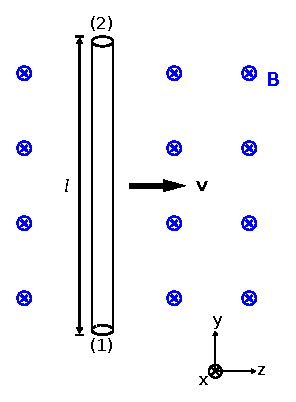
\includegraphics[width=1.75in]{modules/m0059_fStraightWireInB.eps} 
% https://commons.wikimedia.org/wiki/ ...
}}{An x-y-z coordinate system with y vertical, z horizontal, and x going into the page. A wire of length small l is moving at velocity small v in the positive z direction. It moves through a  magnetic field, boldface capital B, shown going into the page. }
\end{center}
\centerline{\scriptsize 
\copyright~\hyperref[m0059_fStraightWireInB_Credit]{C.\ Wang} 
\href{https://creativecommons.org/licenses/by-sa/4.0/}{CC BY 4.0} 
} % \centerline 
\caption{
\label{m0059_fStraightWireInB}
A straight wire moving through a magnetic field.
}
\end{figure}
%
Here, a straight perfectly-conducting wire of length $l$ is parallel to the $y$ axis and moves at speed $v$ in the $+z$ direction through a magnetic field ${\bf B}=\hat{\bf x}B$.
Thus,
%
\begin{flalign}
{\bf v} \times {\bf B} &= \hat{\bf z}v \times \hat{\bf x}B \nonumber \\
                       &= \hat{\bf y} B v
\end{flalign}
%
Taking endpoints 1 and 2 of the wire to be at $y=y_0$ and $y=y_0+l$, respectively, we obtain
%
\begin{flalign}
V_{21} &= \int_{y_0}^{y_0+l} \left[ \hat{\bf y} B v \right] \cdot \hat{\bf y}dy \nonumber \\
       &= Bvl
\end{flalign}
%
Thus, we see that endpoint~2 is at an electrical potential of $Bvl$ greater than that of endpoint~1.
This ``voltage'' exists even though the wire is perfectly-conducting, and therefore cannot be attributed to the electric field.
This voltage exists even though the force required for movement must be the same on both endpoints, or could even be zero, and therefore cannot be attributed to mechanical forces.
Instead, this change in potential is due entirely to the magnetic field. 
  
Because the wire does not form a closed loop, no current flows in the wire.
Therefore, this scenario has limited application in practice.
To accomplish something useful with this concept we must at least form a closed loop, so that current may flow.
For a closed loop, Equation~\ref{m0059_eVAB} becomes:
%
\begin{equation}
V = \oint_{\mathcal C} \left[ {\bf v} \times {\bf B} \right] \cdot d{\bf l}
\label{m0059_eVABc}
\end{equation}
%
Examination of this equation indicates one additional requirement: ${\bf v} \times {\bf B}$ must somehow vary over $\mathcal{C}$.
This is because if ${\bf v} \times {\bf B}$ does not vary over $\mathcal{C}$, the result will be
%
\begin{equation}
\left[ {\bf v} \times {\bf B} \right] \cdot \oint_{\mathcal C} d{\bf l}  \nonumber
\end{equation}
%
which is zero because the integral is zero.
The following example demonstrates a practical application of this idea.

%=--------------------------------

%ORB EXAMPLE
~\\ \begin{example} 
\begin{mdframed}[backgroundcolor=brown!20,linecolor=brown!20]\raggedright
Potential induced in a time-varying loop.
\\~\\
Figure~\ref{m0059_fSlidingBar} shows a modification to the problem originally considered in Figure~\ref{m0059_fStraightWireInB}.
Now, we have created a closed loop using perfectly-conducting and motionless wire to form three sides of a rectangle, and assigned the origin to the lower left corner.
An infinitesimally-small gap has been inserted in the left ($z=0$) side of the loop and closed with an ideal resistor of value $R$.
As before, ${\bf B}=\hat{\bf x}B$ (spatially uniform and time invariant) and ${\bf v}=\hat{\bf z}v$ (constant).
What is the voltage $V_T$ across the resistor and what is the current in the loop?

{\bf Solution.} 
Since the gap containing the resistor is infinitesimally small, 
%
\begin{equation}
V_T = \oint_{\mathcal C} \left[ {\bf v} \times {\bf B} \right] \cdot d{\bf l}
\end{equation}
%
where $\mathcal{C}$ is the perimeter formed by the loop, beginning at the ``$-$'' terminal of $V_T$ and returning to the ``$+$'' terminal of $V_T$.
Only the shorting bar is in motion, so ${\bf v}=0$ for the other three sides of the loop.
Therefore, only the portion of $\mathcal{C}$ traversing the shorting bar contributes to $V_T$.
Thus, we find
%
\begin{equation}
V_T = \int_{y=0}^{l} \left[ \hat{\bf z}v \times \hat{\bf x}B \right] \cdot \hat{\bf y}dy = Bvl
\end{equation}
%
This potential gives rise to a current $Bvl/R$, which flows in the counter-clockwise direction.
\end{mdframed}
%
\begin{figure} % <--- "[b]" for first figure in section *only*; delete for 2nd and subsequent figures
\begin{center}
\pdftooltip{{  % note double braces
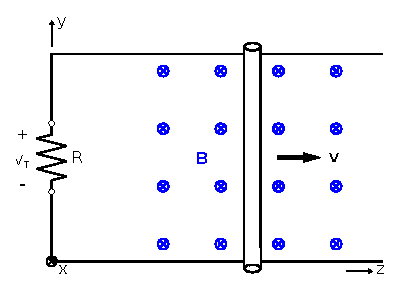
\includegraphics[width=2.5in]{modules/m0059_fSlidingBar.eps} 
% https://commons.wikimedia.org/wiki/ ...
}}{A magnetic field boldface B is into the page. A resistor capital R oriented vertically is part of a square loop of wire of infinite length. A voltage, capital V sub capital T is measured across the resistor from top (positive) to bottom (negative). A cylindrical bar moves with velocity small v away from the resistor in the positive z direction.}
\end{center}
\centerline{\scriptsize 
\copyright~\hyperref[m0059_fSlidingBar_Credit]{C.\ Wang} 
\href{https://creativecommons.org/licenses/by-sa/4.0/}{CC BY-SA 4.0} 
} % \centerline 
\caption{
\label{m0059_fSlidingBar}
A time-varying loop created by moving a ``shorting bar'' along rails comprising two adjacent sides of the loop.
}
\end{figure}
%
\end{example}

Note in the previous example that the magnetic field has induced $V_T$, not the current.  The current is simply a response to the existence of the potential, regardless of the source.  In other words, the same potential $V_T$ would exist even if the gap was not closed by a resistor. 

~\\ %%% FORMATTING KLUDGE

Astute readers will notice that this analysis seems to have a lot in common with Faraday's law,
\index{Faraday's law}
%
\begin{equation}
V = -\frac{\partial}{\partial t}\Phi
\end{equation}
%
which says the potential induced in a single closed loop is proportional to the time rate of change of magnetic flux $\Phi$, where
%
\begin{equation}
\Phi = \int_{S} {\bf B} \cdot d{\bf s}
\end{equation}
%
and where $\mathcal{S}$ is the surface through which the flux is calculated.
From this perspective, we see that Equation~\ref{m0059_eVABc} is simply a special case of Faraday's law, pertaining specifically to ``motional emf.''
\index{motional emf}
Thus, the preceding example can also be solved by Faraday's law, taking $\mathcal{S}$ to be the time-varying surface bounded by $\mathcal{C}$. 

